\documentclass[border=1cm,tikz]{standalone}
\usepackage{amsmath}

\usetikzlibrary{arrows.meta}

\definecolor{lightblue}{rgb}{0.149,0.545,0.824}
\definecolor{superlightcyan}{rgb}{0.9, 1.00, 1.00}
\definecolor{darkblue}{rgb}{0.000, 0.275, 0.545}
\definecolor{darkred}{rgb}{0.647,0.129,0.149}
\definecolor{green}{rgb}{0.365, 0.592, 0.157}

\begin{document}

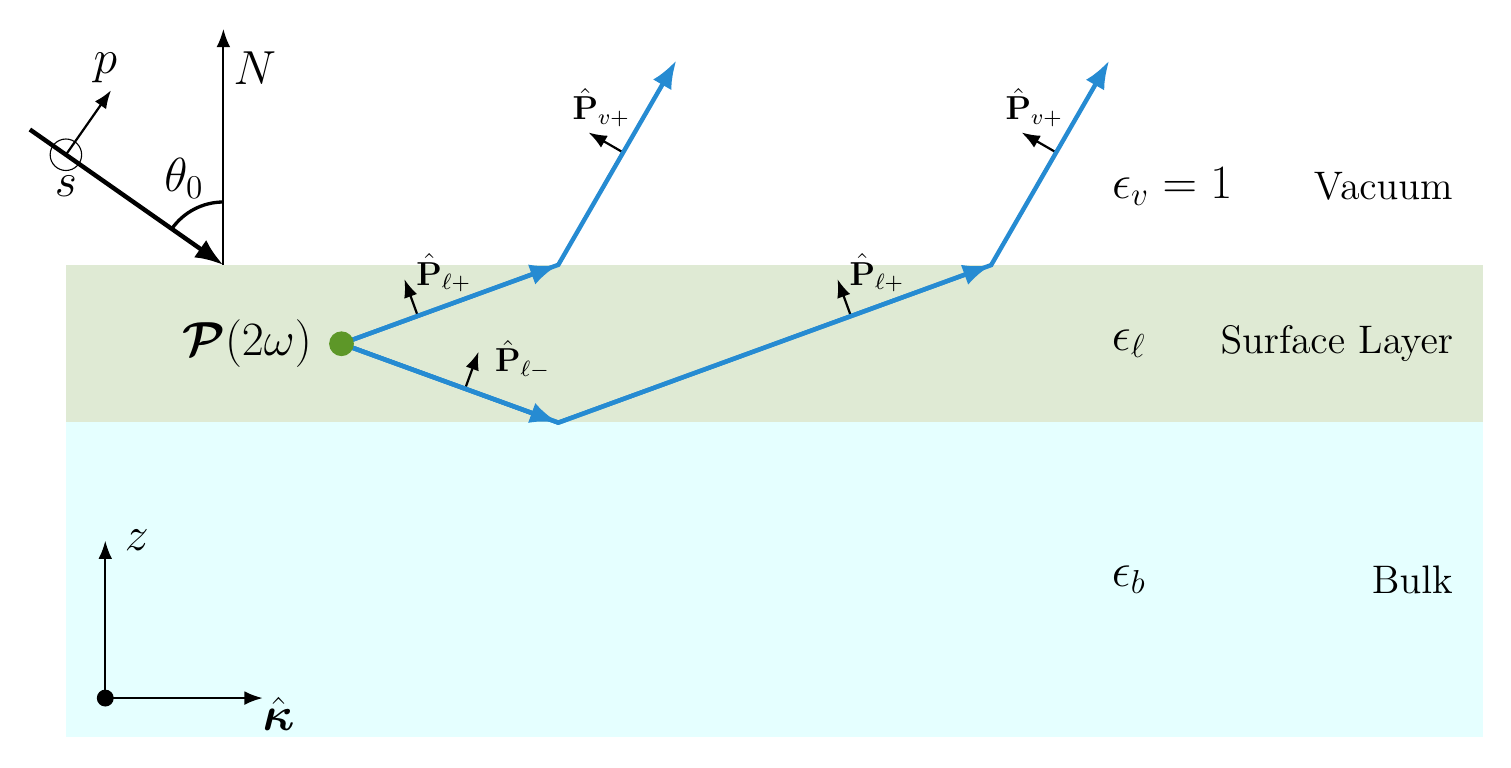
\begin{tikzpicture}

% surface
\fill [superlightcyan] (0,2) rectangle (18,6);
\fill [green,opacity=0.2] (0,6) rectangle (18,8);
%% side labels
\node at (14.05,9) {\LARGE $\epsilon_{v} = 1$};
\node at (16.73,9) {\Large Vacuum};
\node at (13.5,7) {\LARGE $\epsilon_{\ell}$};
\node at (16.14,7) {\Large Surface Layer};
\node at (13.5,4) {\LARGE $\epsilon_{b}$};
\node at (17.1,4) {\Large Bulk};

%% axes
% upper
\draw [very thick] (2,8) +(90:0.8) arc (90:145:0.8);
\node at (1.5,9.1) {\LARGE $\theta_{0}$};
\draw [-Latex,thick] (2,8) -- ++(0,+3);
\node at (2.4,10.5) {\LARGE $N$};
\draw [Latex-,ultra thick] (2,8) -- ++(145:3);
\draw [color=black] (0,9.4) circle (0.20);
\draw [-Latex,thick] (0,9.4) -- ++(55:1);
\node at (0.5,10.5) {\LARGE $p$};
\node at (0,9) {\LARGE $s$};
% lower
\draw [Latex-Latex,thick] (0.5,4.5) -- ++(0,-2) -- ++(2,0);
\filldraw  (0.5,2.5) circle (0.10);
\node at (0.9,4.5) {\LARGE $z$};
\node at (2.7,2.3) {\LARGE $\hat{\boldsymbol{\kappa}}$};

%% inside
% P_{\ell +} and P_{\ell -}
\draw [-Latex,thick] (4.6,6.6) -- ++(-20:0.5) -- ++(70:0.5);
\node at (5.8,6.8) {\large $\hat{\mathbf{P}}_{\ell -}$};
\draw [-Latex,thick] (4,7.18) -- ++(20:0.5) -- ++(110:0.5);
\node at (4.8,7.9) {\large $\hat{\mathbf{P}}_{\ell +}$};
\draw [-Latex,thick] (9.5,7.18) -- ++(20:0.5) -- ++(110:0.5);
\node at (10.3,7.9) {\large $\hat{\mathbf{P}}_{\ell +}$};
\draw [-Latex,thick] (6.82,9) -- ++(60:0.5) -- ++(150:0.5);
\node at (12.3,10) {\large $\hat{\mathbf{P}}_{v +}$};
\draw [-Latex,thick] (12.32,9) -- ++(60:0.5) -- ++(150:0.5);
\node at (6.8,10) {\large $\hat{\mathbf{P}}_{v +}$};
% first beam from the left
\node at (2.3,7) {\LARGE $\boldsymbol{\mathcal{P}}(2\omega)$};
\draw [-Latex,ultra thick,lightblue] (3.5,7) -- ++(20:2.93);
\draw [-Latex,ultra thick,lightblue] (3.5,7) -- ++(20:2.93) -- ++(60:3);
\draw [-Latex,ultra thick,lightblue] (3.5,7) -- ++(-20:2.93);
\draw [-Latex,ultra thick,lightblue] (3.5,7) -- ++(-20:2.93) -- ++(20:5.85);
\draw [-Latex,ultra thick,lightblue] (3.5,7) -- ++(-20:2.93) -- ++(20:5.85) -- ++(60:3);
\filldraw [green] (3.5,7) circle (0.15);

\end{tikzpicture}

\end{document}
